\lecture{Gestione Delle Scorte}{13~-~02~-~2026}
%
\section{Rilevanza Economica e Aziendale}
La gestione dei materiali e delle scorte rappresenta un pilastro fondamentale per l'efficienza operativa e la salute finanziaria di qualsiasi realtà aziendale. Una corretta pianificazione non solo ottimizza i flussi produttivi, ma incide direttamente sulla redditività e sulla competitività nel mercato.

L'impatto delle scorte si manifesta sia a livello macroeconomico che microeconomico:
\begin{itemize}
    \item \textbf{Impatto sul PIL}: Il valore delle scorte rappresenta circa il 15\% del PIL, con un costo finanziario annuo stimato al 10\%. Complessivamente, la gestione dei materiali ``brucia'' oltre il 5\% del PIL.
    \item \textbf{Effetti sul Bilancio}: Sebbene le scorte incrementino l'attivo dello stato patrimoniale, esse comportano una diminuzione dei profitti e degli indici di redditività, aumentando contestualmente gli indici di indebitamento.
\end{itemize}

%
\subsection{Indicatori di Prestazione}
Per misurare l'efficienza della gestione, è essenziale monitorare la velocità con cui i materiali circolano in azienda
%
\paragraph{Indice di Rotazione (Turnover)} Rapporto tra il fatturato (domanda per valore unitario) e il valore medio delle scorte.
\[
    \text{Turnover} = \frac{\text{Fatturato}}{\text{Valore Medio delle Scorte}}
\]
%
\paragraph{Indice di Giacenza Media} Rappresenta l'inverso del turnover, indica il tempo medio di permanenza dei materiali in magazzino.
\[
    I_{\text{GM}} = \frac{1}{\text{Turnover}}
\]
%
\paragraph{Altre formule utili} Adesso elenco altre formule utili per i calcoli riguardanti i magazzini, tra cui:
\begin{itemize}
    \item il Fatturato $ F $;
    \item la quantità media magazzino $ QM $;
    \item il valore medio delle scorte $ VS $.
\end{itemize}
\begin{gather*}
    F = \text{Domanda} \cdot \text{Valore}                            \\
    QM = \frac{\text{Dimensione Ordine}}{2} \\
    VM = QM \cdot \text{Valore}
\end{gather*}

\begin{example}[Indice di Turnover]
    Un'azienda ha una domanda annuale di 10.000 pezzi di valore unitario \euro{50} che soddisfa mediante ordini trimestrali.

    Calcolare gli indici di prestazione delle scorte.

    \begin{gather*}
        F = d \cdot v = 10000 \cdot 50 = 5 \cdot 10^{5} \text{\euro} \\
        VS = (\frac{\text{Dimensione Ordine}}{2}) \cdot v = (\frac{\frac{10000}{4}}{2}) \cdot 50 = 6.25 \cdot 10^{4} \text{\euro} \\
        \text{Turnover} = \frac{5 \cdot 10^{5}}{6.25 \cdot 10^{4}}= 8 \\
        I_{GM} = \frac{1}{\text{Turnover}} = \frac{1}{8} = 0.125
    \end{gather*}
\end{example}

%
\section{Politiche e Tipologie di Scorta}
La decisione su quando e quanto ordinare risponde a diverse logiche strategiche:
\begin{itemize}
    \item \textbf{Motivazioni Economiche}
          \begin{itemize}
              \item \emph{Costi di transazione}: Distribuzione dei costi fissi su un volume maggiore di prodotti;
              \item \emph{Prudenza}: Costituzione di scorte di sicurezza per tutelarsi contro le incertezze delle quantità;
              \item \emph{Speculazione}: Acquisto anticipato per proteggersi da possibili aumenti di prezzo.
          \end{itemize}
    \item \textbf{Classificazione Funzionale}: Le scorte possono essere classificate in base al loro ruolo nel ciclo produttivo: materie prime, semilavorati (Work in Process), prodotti finiti e ricambi. Tra le tipologie funzionali si distinguono:
          \begin{itemize}
              \item Scorta di ciclo, di congestione, di sicurezza, di anticipazione, di flusso e di disaccoppiamento.
          \end{itemize}
\end{itemize}

%
\section{Sistemi di Osservazione e Classificazione ABC}
Il monitoraggio può avvenire secondo due modalità principali:
\begin{enumerate}
    \item \textbf{Continuous Review System (Sistema Q)}: Il livello viene controllato a ogni singolo prelievo.
    \item \textbf{Periodic Review System (Sistema P)}: Il controllo avviene a intervalli di tempo prefissati.
\end{enumerate}

%
\subsection{Analisi ABC (Legge di Pareto)}
Non tutti gli articoli (SKU~-~Stock Keeping Unit) hanno lo stesso peso economico. La classificazione ABC permette di focalizzare l'attenzione sugli elementi critici:

\begin{itemize}
    \item \textbf{Classe A}: Pochi articoli (5-10\%) che generano la maggior parte del valore (75-80\%);
    \item \textbf{Classe B}: Articoli intermedi (10-15\%) con un valore del 10-15\%;
    \item \textbf{Classe C}: La maggioranza degli articoli (80\%) che pesa solo per il 10\% del valore totale.
\end{itemize}

%
\section{Dinamica e Simulazione dei Costi} \label{sec:dinamica_sim}
Il livello dell'inventario ($I_t$) è regolato dalla legge di conservazione:
\begin{gather*}
    I_t = I_{t-1} + a_t - u_t \\
    I_{t}\geq 0, \quad \forall t \geq 0
\end{gather*}

dove $ I_{t} $ è il livello dell'inventario, $ t $ è il tempo, $a_t$ rappresenta gli arrivi (forniture) e $u_t$ le uscite (consegne).

Se $ t=0 $, allora:
\[
    I_{0} = I^{0}
\]
dove $ I^{0} $ rappresenta il livello iniziale.

Nella valutazione dei costi totali di gestione, occorre considerare tre componenti fondamentali:
\begin{enumerate}
    \item \textbf{Costo del prodotto}: Valore di acquisto dei beni consegnati;
    \item \textbf{Costo di stoccaggio} ($h$): Onere per mantenere la merce a magazzino per unità di tempo;
    \item \textbf{Costo di ordinazione} ($A$): Costo fisso associato all'emissione di ogni ordine di acquisto;
\end{enumerate}

%
\section{Domanda costante e deterministica}
In questa sezione affronteremo le logiche matematiche e aziendali che ci guidano nel rispondere a due domande cruciali: quanto ordinare e quando ordinare in condizioni di certezza assoluta.
%
\subsection{Ipotesi modello base}
Per analizzare correttamente la dinamica di un magazzino, dobbiamo prima definire il nostro vocabolario di base:
\begin{itemize}
    \item $T$: Periodo di tempo considerato;
    \item $D$: Domanda del prodotto in unità;
    \item $Q$: Dimensione del lotto (o ordine) in unità;
    \item $c$: Costo unitario del prodotto (Euro/unità);
    \item $A$: Costo di ordinazione o setup (Euro per singolo ordine);
    \item $h$: Costo unitario di stoccaggio (Euro/unità per periodo);
    \item $r$: Costo finanziario unitario di stoccaggio espresso in percentuale.
\end{itemize}
Il modello matematico di base si fonda su alcune ipotesi restrittive:
\begin{itemize}
    \item \textbf{Domanda deterministica}: Non vi è incertezza sulla quantità o sulla tempistica della domanda;
    \item \textbf{Domanda costante nel tempo}: Può essere rappresentata mediante una linea retta;
    \item \textbf{Produzione istantanea}: Non vi sono vincoli di capacità produttiva e il lotto viene prodotto istantaneamente;
    \item \textbf{Consegna immediata}: Non vi sono ritardi tra la produzione e la disponibilità a soddisfare la domanda;
    \item \textbf{Costo di ordinazione costante}: Non dipende dalla dimensione del lotto o dallo stato del sistema produttivo;
    \item \textbf{Analisi di un singolo prodotto}: Non si deve tener conto di possibili interazioni con altri prodotti;
    \item \textbf{Prezzo costante}: Non dipende dalla dimensionsione del lotto.
\end{itemize}

\begin{figure}
    \centering
    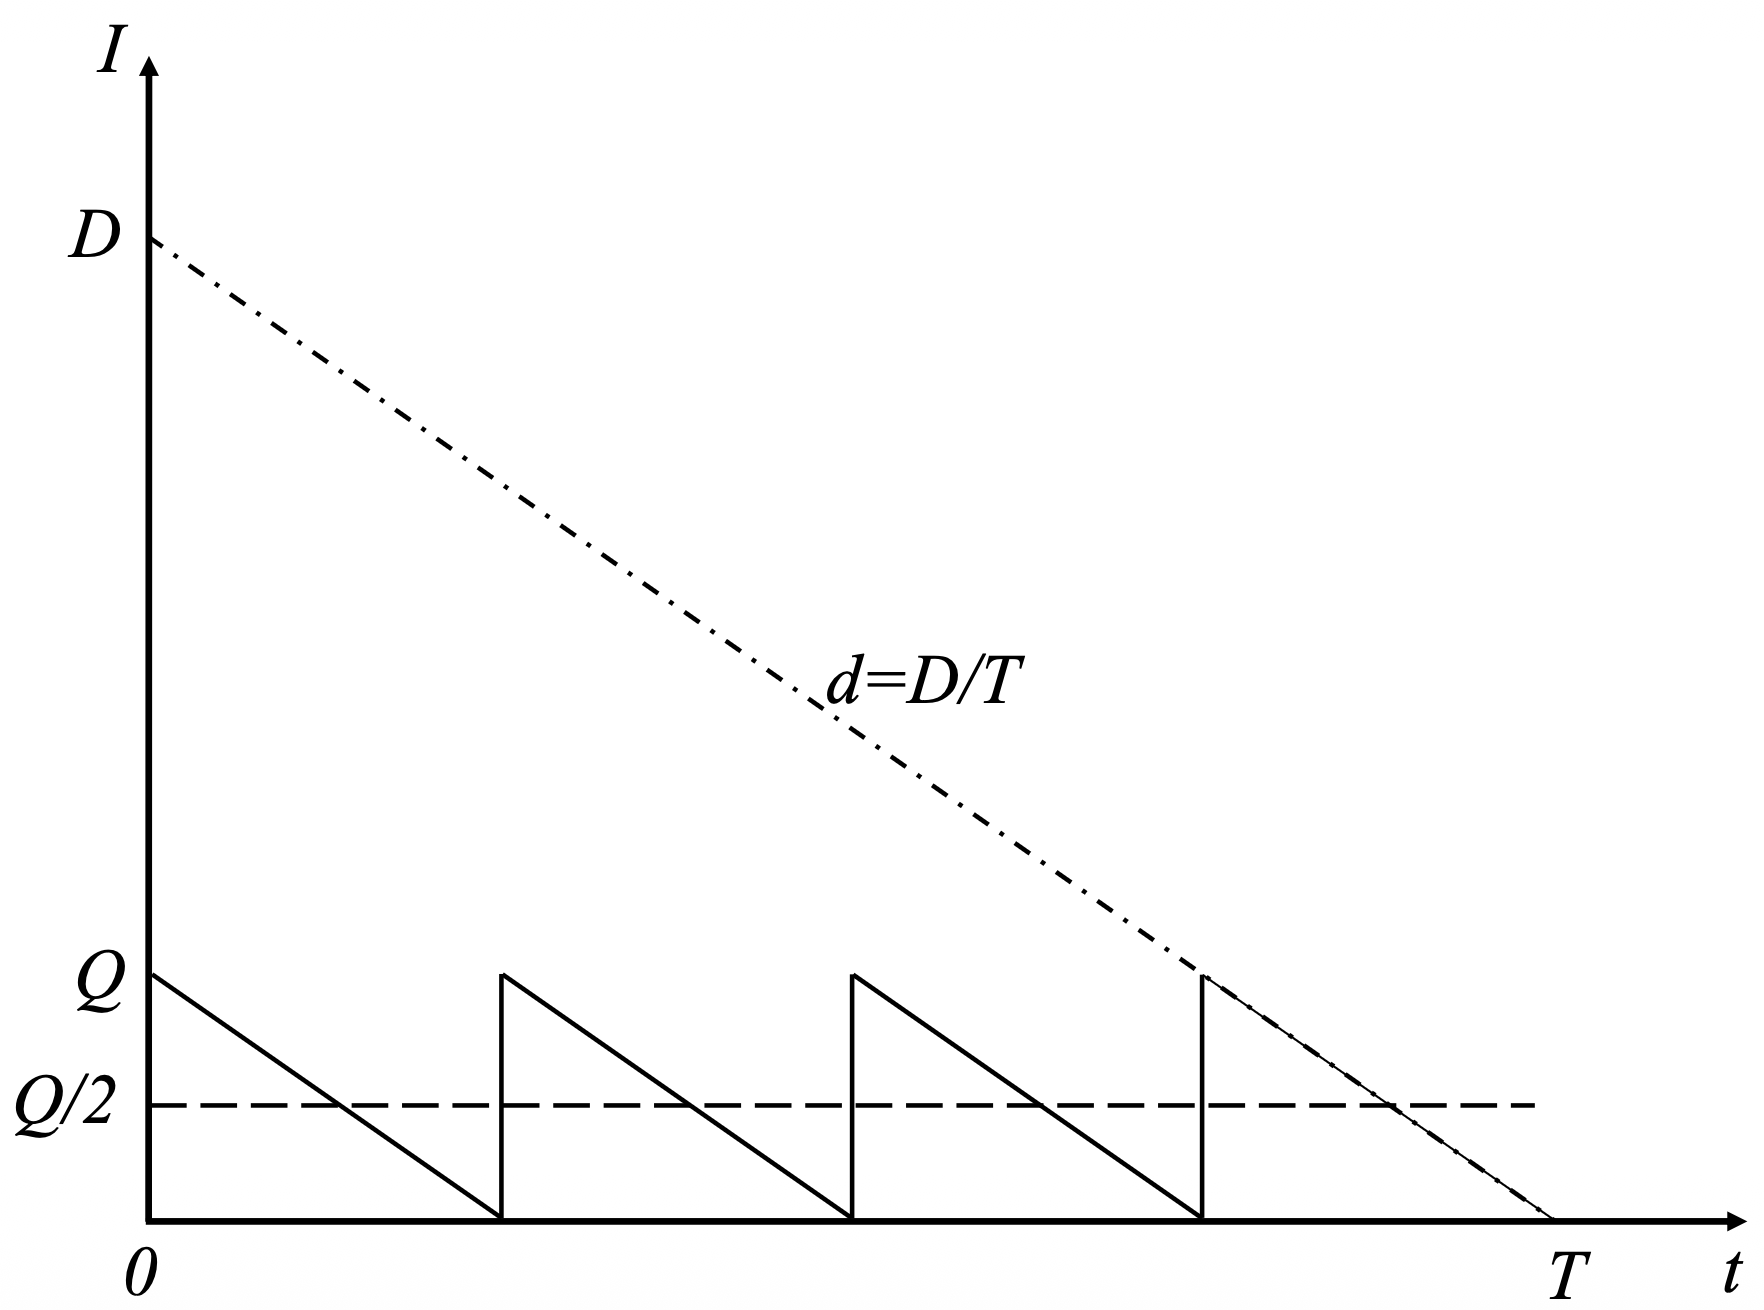
\includegraphics[width=0.4\linewidth]{assets/Screenshot 2026-02-14 at 15.57.07.png}
    \caption{Dinamica dei magazzini}\label{fig:.}
\end{figure}

%
\subsection{Funzione di costo totale}
La gestione ottimale mira a minimizzare il Costo Totale (TC) dell'inventario, che si compone di tre voci fondamentali:
\[
    TC = cD + A \frac{D}{Q} + h \frac{Q}{2}
\]
\begin{enumerate}
    \item \textbf{Costo totale di acquisto} ($cD$): Una quantità costante, dato che l'intera domanda annuale deve essere comunque soddisfatta;
    \item \textbf{Costo totale di ordinazione} ($A\frac{D}{Q}$): Diminuisce all'aumentare della quantità ordinata $Q$, poiché faremo meno ordini all'anno;
    \item \textbf{Costo totale di stoccaggio} ($h\frac{Q}{2}$): Aumenta linearmente all'aumentare di $Q$, calcolato sull'inventario medio ($Q/2$).
\end{enumerate}
A riguardo vedi figura \ref{fig:ddin}.
\begin{figure}
    \centering
    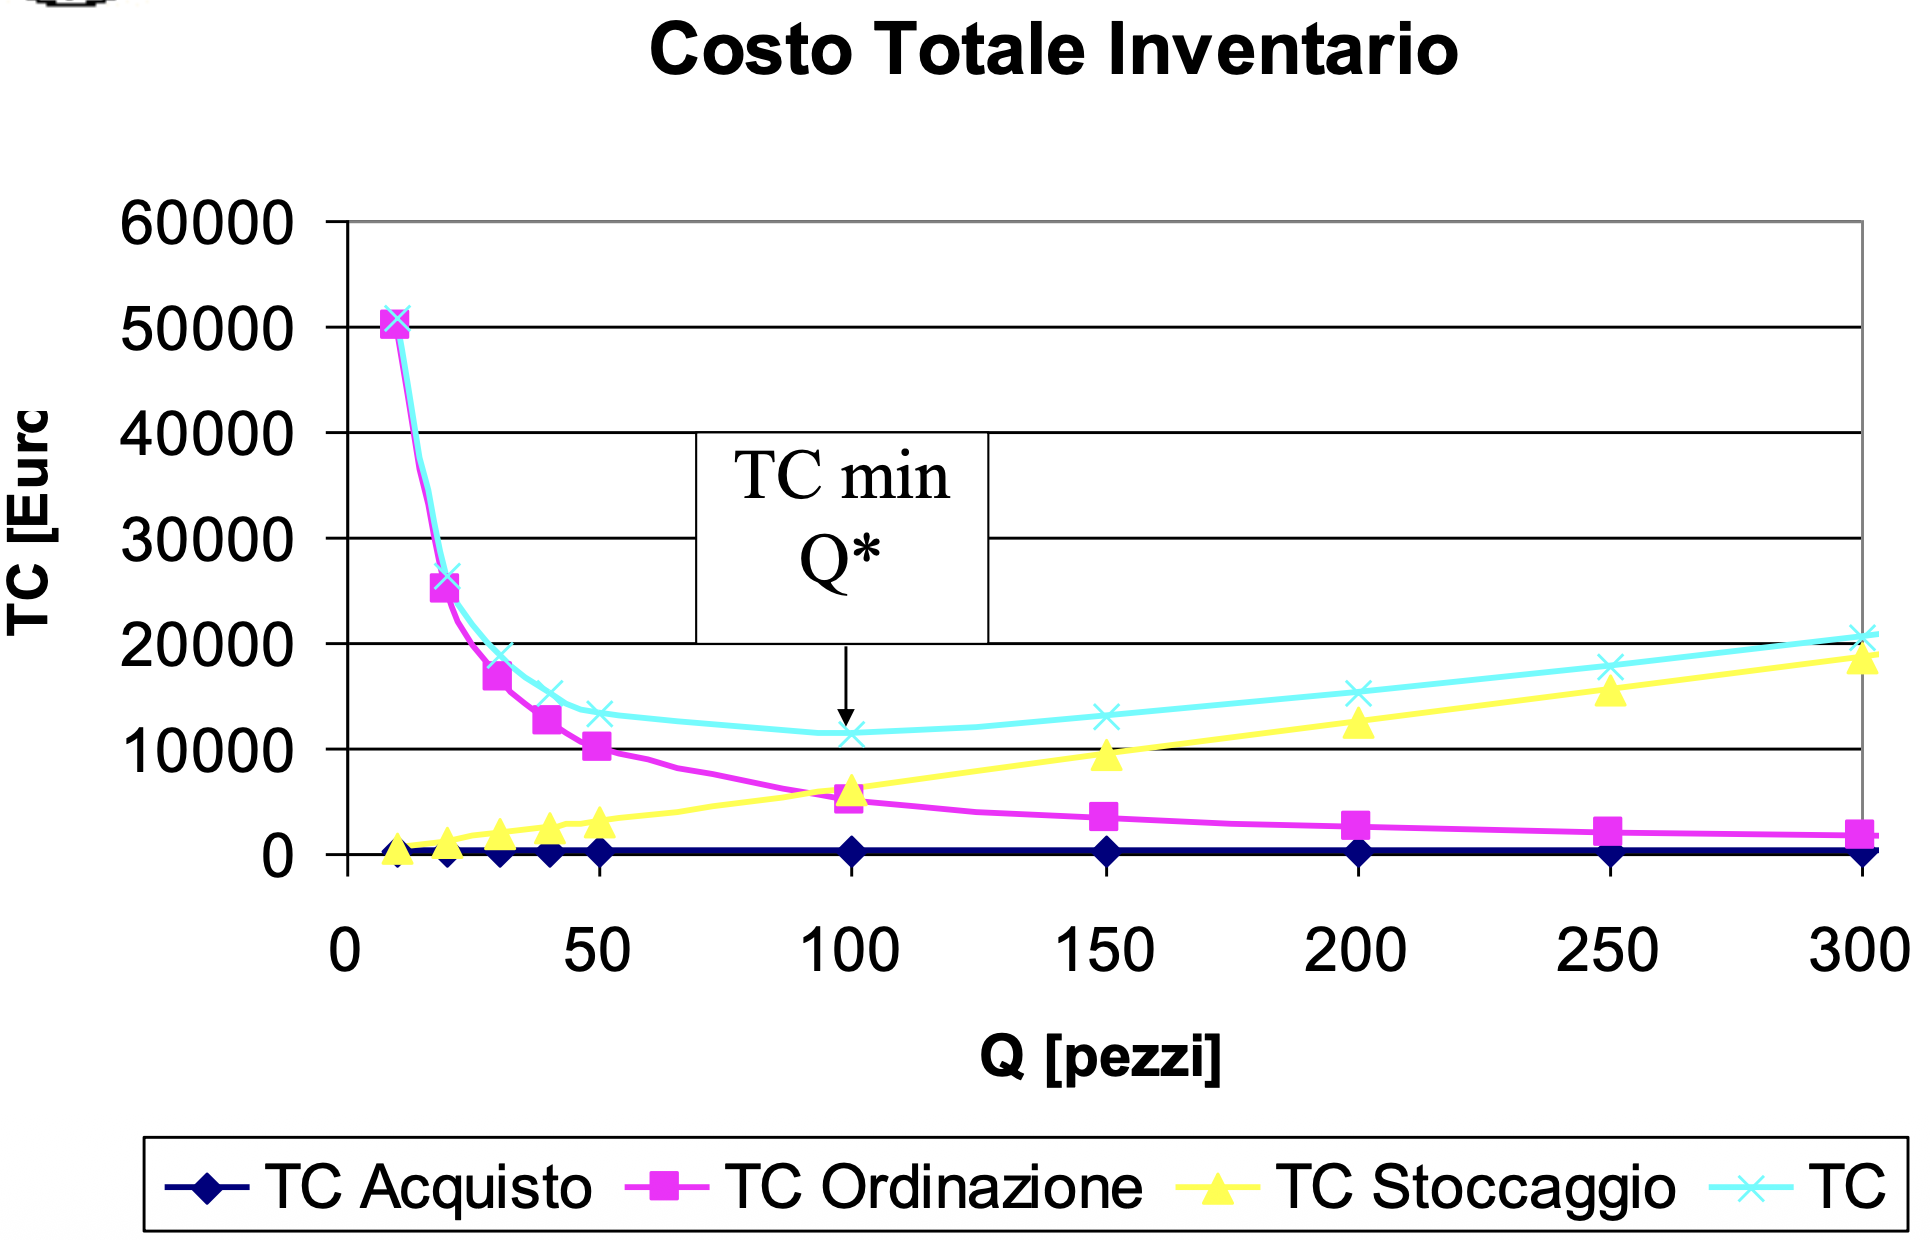
\includegraphics[width=0.6\linewidth]{assets/Screenshot 2026-02-14 at 16.00.43.png}
    \caption{Funzione di costo totale}\label{fig:ddin}
\end{figure} \clearpage

%
\section{Economic Order Quantity}
L'obiettivo è trovare quel valore della quantità ordinata $Q$ che minimizza il costo totale. Derivando la funzione $TC$ rispetto a $Q$ e ponendola uguale a zero, otteniamo la formula del \emph{Lotto Economico}.

\begin{gather*}
    TC = cD + A \frac{D}{Q} + h \frac{Q}{2} \\
    \frac{\partial TC}{\partial Q} = - \frac{AD}{Q^{2}}+\frac{h}{2} = 0 \\
    Q^{*}=\sqrt{\frac{2AD}{h}}
\end{gather*}
Sostituendo $ Q^{*} $ nella funzione di partenza, il \emph{Costo Totale Ottimo} risulta essere:
\begin{gather*}
    Q^{*}=\sqrt{\frac{2AD}{h}} \qquad TC = cD + A \frac{D}{Q} + h \frac{Q}{2} \\
    TC = cD + A \frac{D}{\sqrt{\frac{2AD}{h}}} + h \frac{\sqrt{\frac{2AD}{h}}}{2} = \\
    = cD + \sqrt{\frac{ADh}{2}} + \sqrt{\frac{ADh}{2}} = cD + \sqrt{2ADh}
\end{gather*}
possiamo concludere quindi:
\[
    TC^{*} = cD + \sqrt{2ADh}
\]

\begin{note}[Variabile costo]
    Fare attenzione: spesso il costo $h$ include una componente fissa e una finanziaria, calcolata come $h + rc$.
\end{note}

%
\subsection{Sensitività dell'EOQ}
Se $ Q_{1} = 2Q^{*} $, allora:
\[
    TC_{1} = cD + \sqrt{2ADh} + \frac{1}{4} \sqrt{2ADh}
\]
Se $ Q_{2} = \frac{1}{2}Q^{*} $, allora:
\[
    TC_{2} = cD + \sqrt{2ADh} + \frac{1}{4}\sqrt{2ADh}
\]

%
\subsection{Lead Time e livello di riordino}
Se abbandoniamo l'ipotesi di consegna immediata, dobbiamo introdurre il Lead Time ($LT$), ovvero il tempo di attesa per la consegna. Bisogna quindi emettere l'ordine prima di esaurire le scorte, precisamente al raggiungimento di un Livello di riordino $R$.

\[
    R = d \cdot LT
\]

Per il calcolo di $R$ abbiamo utilizziamo il tasso di domanda $d = D/T$, questo vuol dire che:
\[
    R = \frac{D}{T} \cdot LT
\]
dove $ D $ è la domanda (es. 1000 contenitori) e $ T $ è il tempo (es. anno).
\begin{example}[Lead Time]
    Un'azienda utilizza annualmente 1000 contenitori che acquista da un
    fornitore al prezzo di 250 Euro.
    \begin{itemize}
        \item Definire il livello di riordino sapendo che il lead time del fornitore è di 7 giorni;
    \end{itemize}
    \[
        R = \frac{D}{T} \cdot LT = \frac{1000}{365} \cdot 7 \approx 20 \si{p}
    \]
\end{example}


Se il Lead Time è inferiore al ciclo di riordino, utilizziamo la formula appena vista. Se il Lead Time supera un intero ciclo produttivo, si applica la formula più generale che tiene conto dei lotti già in arrivo:

\[
    R = d \cdot LT - \lfloor \frac{d \cdot LT}{EOQ} \rfloor \cdot EOQ
\]

In questa fase è cruciale distinguere tra Giacenza (materiale fisicamente in magazzino) e Disponibilità (giacenza + ordini a fornitore - ordini cliente), poiché è la disponibilità che comanda lo scatto del riordino.

\begin{example}[Lead Time]
    Un'azienda utilizza annualmente 1000 contenitori che acquista da un
    fornitore al prezzo di 250 Euro. Il costo di ordinazione è di 500 Euro mentre il costo unitario annuale di immagazzinamento è la somma del costo di occupazione del magazzino, 100 Euro all'anno, e dall'interesse (10\%) sul capitale impegnato per l'acquisto del contenitore.
    \begin{itemize}
        \item Definire il livello di riordino sapendo che il lead time del fornitore è di 42 giorni;
    \end{itemize}
    \begin{gather*}
        R = \frac{D}{T} \cdot LT - \lfloor \frac{d \cdot LT}{EOQ} \rfloor \cdot EOQ \\
        R = \frac{1000}{365} \cdot 42 - \lfloor \frac{2.74 \cdot 42}{90} \rfloor \cdot 90 = 2.74 \cdot 42 - 1 \cdot 90 \approx 25 \si{p}
    \end{gather*}
    \begin{itemize}
        \item Definire il livello di riordino sapendo che il lead time del fornitore è di 70 giorni.
    \end{itemize}
    \begin{gather*}
        R = \frac{D}{T} \cdot LT - \lfloor \frac{d \cdot LT}{EOQ} \rfloor \cdot EOQ \\
        R = \frac{1000}{365} \cdot 70 - \lfloor \frac{2.74 \cdot 70}{90} \rfloor \cdot 90 = 2.74 \cdot 70 - 2 \cdot 90 \approx 12 \si{p}
    \end{gather*}
\end{example}

%
\section{Economic Manufacturing Quantity}
Se siamo noi a produrre il bene internamente, il lotto non arriva tutto in un istante, ma con un \emph{tasso di produzione} ($p$) graduale. Nel frattempo, continuiamo a consumare il bene al \emph{tasso di domanda} ($d$). Il magazzino si riempirà quindi a un tasso netto $r = p - d$.

Il livello massimo di magazzino ($I_m$) non sarà più $Q$, bensì:
\[
    I_m = (p-d) \cdot T_{p}
\]
dove $ T_{p} $ è il periodo di produzione, calcolato tramite:
\[
    T_{p} = \frac{Q}{p}
\]
allora:
\[
    I_{m} = Q \frac{p-d}{p}
\]
La formula del lotto ottimo di produzione (\textbf{EMQ}) viene modificata includendo questo rapporto:
\begin{align*}
    TC     & = cD + A \frac{D}{Q} + h \frac{I_{m}}{2}           \\
    TC     & = cD + A \frac{D}{Q} + h \frac{Q}{2} \frac{p-d}{p} \\
    Q^{*}  & = \sqrt{\frac{2AD}{h}} \sqrt{\frac{p}{p-d}}        \\
    TC^{*} & = cD + \sqrt{2ADh} \sqrt{\frac{p-d}{p}}
\end{align*}

\begin{example}[EMQ]
    Un'azienda utilizza 12000 inserti di teflon all'anno. Il costo di installazione dell'attrezzatura di produzione è di 50 Euro e la produzione settimanale è di 1000 unità. Il costo unitario dell'inserto è di 1 Euro e il costo di giacenza annuale è di 0,25 Euro per inserto.
    \begin{itemize}
        \item Calcolare la dimensione ottimale del lotto di produzione.
    \end{itemize}
    Dati:
    \begin{gather*}
        d = \frac{D}{T} = \frac{12000}{52} = 231 \ \text{pezzi/settimana} \\
        p = 1000 \ \text{pezzi/settimana}
    \end{gather*}

    Risoluzione:
    \begin{gather*}
        Q^{*}= \sqrt{\frac{2 \cdot 50 \cdot 12000}{0.25}}\sqrt{\frac{1000}{1000-231}} = 2498 \ \text{pezzi} \\
        TC^{*} = cD + \sqrt{2ADh}\sqrt{\frac{p-d}{p}} = 12480 \ \text{\euro}
    \end{gather*}
\end{example}

%
\section{Quantity Discounts}
Spesso i fornitori offrono sconti se acquistiamo lotti maggiori ($Q_1$, $Q_2$). Il prezzo non è più costante ($c$, $c_1$, $c_2$). In questo caso la curva del costo totale presenta dei ``salti'' verso il basso.

Definiamo il costo unitario $ c $, il costo unitario $ c_{1} $ per cui $ Q>Q_{1} $ ed il costo unitario $ c_{2} $ per cui $ Q>Q_{2} $:
\begin{gather*}
    TC = cD + A \frac{D}{Q} + h \frac{Q}{2}~, \qquad     \min
    \begin{Bmatrix}
        TC^{*}, TC_{1}, TC_{2}
    \end{Bmatrix}
\end{gather*}
\begin{align*}
    TC^{*} & = cD + \sqrt{2ADh}                               \\
    TC_{1} & = c_{1}D + A \frac{D}{Q_{1}} + h \frac{Q_{1}}{2} \\
    TC_{2} & = c_{2}D + A \frac{D}{Q_{2}} + h \frac{Q_{2}}{2}
\end{align*}
Vedi figura \ref{fig:disc} a riguardo.

\begin{figure}
    \centering
    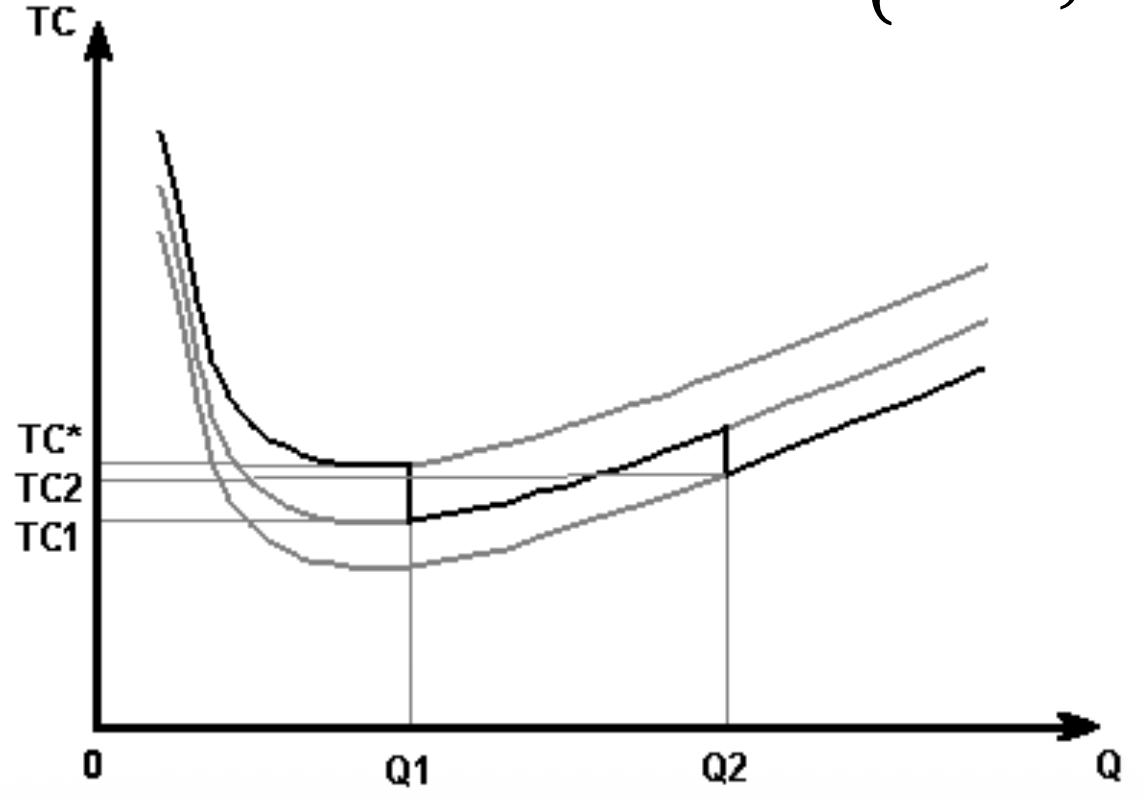
\includegraphics[width=0.5\linewidth]{assets/Screenshot 2026-02-14 at 18.02.49.png}
    \caption{Quantity Discount}\label{fig:disc}
\end{figure}